\subsection{Acquisizione}
Nel $\textit{processo}_G$ di acquisizione avviene la raccolta e la comprensione dei requisiti con lo scopo di identificare un $\textit{capitolato}_G$ adeguato per il gruppo da proporre per la $\textit{candidatura}_G$.
\subsubsection{Valutazione capitolati}
Il gruppo ha analizzato la proposta dei proponenti valutandone, in base all'esperienza del gruppo, la loro \textit{complessità}; tale analisi è stata determinante per la scelta definitiva.
\subsubsection{Appalto capitolati}
Il gruppo si è proposto per il $\textit{capitolato}_G$ C3 dell'azienda $\textit{Imola Informatica}_G$. Nonostante un  un primo riscontro negativo, a seguito di modifiche volte a sistemare lacune presenti  presenti nella $\textit{candidatura}_G$ iniziale, il gruppo è riuscito ad aggiudicarsi il $\textit{capitolato}_G$.

\subsection{Fornitura}
Il $\textit{processo}_G$ di $\textit{fornitura}_G$ consiste nel chiarire ogni dubbio legato al prodotto finale che il proponente desidera; in modo da evitare incomprensioni durante lo svolgimento del progetto, il gruppo RAMtastic6 si impegna a comunicare con l'azienda, in modo da raggiungere i seguenti obiettivi:
\begin{enumerate}
    \item Determinare i requisiti da soddisfare nel prodotto finale;
    \item Ottenere incontri di formazioni sulle $\textit{tecnologie}_G$ e strumenti consigliati dall'azienda per realizzare il prodotto;
    \item Ricevere $\textit{feedback}_G$ in fase di sviluppo su quanto precedentemente svolto.
\end{enumerate}

\subsubsection{Lettera di Presentazione}
La \textit{Lettera di Presentazione} è il documento che fornisce la presentazione della documentazione e del prodotto durante le varie fasi di revisione di progetto. 
\\
Questo documento riporta l’insieme della documentazione richiesta che sarà consegnata ai committenti, il Prof. Tullio Vardanega e il Prof. Riccardo Cardin.

\subsubsection{Analisi dei Requisiti v3.0.0}
L'\textit{Analisi dei Requisiti} stabilisce una comprensione comune tra gli \textit{stakeholder} riguardo alle caratteristiche e alle prestazioni del $\textit{software}_G$ da sviluppare. Questo documento elimina le ambiguità che potrebbero sorgere durante la comunicazione e fornisce una base chiara per il progetto.
\\
Il documento di \textit{Analisi dei Requisiti} è strutturato in diverse sezioni chiave:
\begin{itemize}
\item \textbf{Introduzione}: Fornisce una panoramica generale del prodotto e delle sue funzionalità principali. Questa sezione stabilisce il contesto per il resto del documento e fornisce una visione d'insieme del progetto.

\item \textbf{Casi d'uso}: Identifica e descrive tutti i possibili scenari di utilizzo del $\textit{software}_G$ da parte degli utenti. Ogni $\textit{caso d'uso}_G$ descrive un'interazione specifica tra l'utente e il $\textit{sistema}_G$, illustrando come il $\textit{software}_G$ dovrebbe essere utilizzato per soddisfare le esigenze degli utenti.

\item \textbf{Requisiti}: Raccoglie tutte le richieste e i vincoli definiti dal cliente o emersi durante le discussioni con il team di sviluppo. Ogni $\textit{requisito}_G$ è accompagnato da una descrizione dettagliata che specifica ciò che il $\textit{sistema}_G$ deve fare o quale comportamento deve avere. Questi requisiti costituiscono la base per la progettazione e lo sviluppo del $\textit{software}_G$.
\end{itemize}

\subsubsection{Specifica Tecnica v1.0.0}
Il documento \textit{Specifica Tecnica} descrive in modo dettagliato le scelte progettuali effettuate dal gruppo per la realizzazione del $\textit{sistema}_G$ richiesto dal proponente. 
\\Viene compresa l’architettura logica e l’architettura di \textit{deployment} oltre che la lista
delle $\textit{tecnologie}_G$ utilizzate e i $\textit{design}_G$ pattern adottati.
Inoltre, viene fornita una sezione relativa al tracciamento dei requisiti soddisfatti in linea con il documento di \textit{Analisi dei Requisiti}.

\subsubsection{Manuale Utente v1.0.0}
Il \textit{Manuale Utente} ha lo scopo di fornire all'utilizzatore del prodotto un orientamento verso quelli che sono tutti gli scenari in cui potrà navigare l'utente una volta messo in atto. \\
Comprende una guida di navigazione completa per eliminare tutti i dubbi che potrebbe avere durante l'utilizzo di tutte le funzionalità che il prodotto ha da offrire.

\subsubsection{Glossario v2.0.0}
Il \textit{Glossario} è il documento alla base di ogni altro documento di supporto. Il suo scopo è quello di esplicitare il significato dei termini comunemente usati all'interno di tutta la documentazione prodotta, al fine di evitare ambiguità o incomprensioni. \\
E' rivolto sia ai componenti del gruppo che ai committenti e ai proponenti. 

\subsubsection{Piano di Progetto v2.0.0}
Il documento \textit{Piano di Progetto} costituisce uno $\textit{strumento}_G$ di pianificazione per tutte le attività che dovranno essere svolte così da poter rispettare la data di consegna del progetto.
Nel dettaglio il $\textit{Piano di Progetto}_G$ è composto da:
\begin{itemize}
    \item $\textit{Analisi Dei Rischi}_G$: analisi delle difficoltà che il gruppo potrebbe riscontrare durante lo svolgimento del progetto, in particolar modo a livello organizzativo e tecnologico;
    \item Modello di sviluppo;
    \item Pianificazione;
    \item $\textit{Preventivo}_G$: che rispecchi quanto comunicato in fase di $\textit{candidatura}_G$;
    \item $\textit{Consuntivo}_G$: tracciamento dell'andamento del gruppo rispetto al $\textit{preventivo}_G$ fatto.
\end{itemize}
\subsubsection{Piano di Qualifica v2.0.0}
Nel documento \textit{Piano di Qualifica} vengono elencate tutte le attività svolte dal verificatore con l'obiettivo di garantire la qualità del prodotto finale.
E' formato dai seguenti componenti:
\begin{itemize}
    \item Qualità di processo
    \item Qualità di prodotto
    \item $\textit{Test}_G$: eseguiti sul prodotto che assicurano che i requisiti siano stati rispettati
    \item Resoconto
\end{itemize}
\subsubsection{Rilascio}
Quando il prodotto verrà ultimato, verrà collaudato per garantire il suo corretto funzionamento. Se il prodotto supera il collaudo, verrà consegnato al committente insieme alla documentazione del progetto. 
Il gruppo non effettuerà $\textit{manutenzione}_G$ una volta rilasciato il prodotto.
\subsubsection{Strumenti}
Per il $\textit{processo}_G$ di $\textit{fornitura}_G$ vengono utilizzati i seguenti strumenti:
\begin{itemize}
    \item \emph{\textbf{Microsoft Teams}}: servizio di videoconferenza utilizzato per gli incontri con il proponente;
    \item \emph{\textbf{Telegram}}: servizio di messaggistica utilizzato per le comunicazioni con il proponente;
    \item \emph{\textbf{Share Point}}: servizio che permette di condividere e gestire contenuti Office tramite browser, utilizzato per creare le presentazioni per i diari di bordo.
\end{itemize}

\subsection{Sviluppo}
Lo scopo del $\textit{processo}_G$ di sviluppo è quello di dichiarare le attività da svolgere per raggiungere i requisiti necessari del prodotto.
A tale scopo, il gruppo si dividerà in diversi ruoli, i quali avranno compiti precisi da svolgere.
\subsubsection{Analisi Dei Requisiti}
\textit{Analisi Dei Requisiti} è un documento fondamentale per lo sviluppo. Infatti, tale documento deve indicare i requisiti necessari del prodotto finale, che a loro volta andranno a rispecchiare le aspettative del proponente. \\
Inoltre, questo documento servirà anche come documentazione del prodotto, andandone infatti a contenere tutte le relative Funzionalità.
\subsubsubsection{Attori} 
Innanzitutto, verranno definiti gli attori e una panoramica dei vari casi d'uso a loro associati tramite un diagramma
\subsubsubsection{Casi d'uso}
Successivamente, verranno descritti i vari casi d'uso, i quali hanno il compito di rappresentare le Funzionalità che il prodotto finale dovrà rispettare. \\
I casi d'uso saranno ordinati per $\textit{attore}_G$, ovvero verranno prima descritti tutti i casi d'uso associati a un particolare $\textit{attore}_G$, per poi proseguire con la descrizione di tutti i casi d'uso riguardanti l'$\textit{attore}_G$ successivo, e a proseguire. \\
Ogni Caso d'Uso avrà un diagramma ad esso associato e la sua descrizione $\textit{verbale}_G$. Gli use case cosiddetti "atomici" saranno inseriti nello $\textit{scenario}_G$ principale, il quale rappresenterà le azioni compiute in modo consecutivo dall'$\textit{attore}_G$ nello $\textit{scenario}_G$ più comune. \\
La descrizione $\textit{verbale}_G$ di ogni $\textit{caso d'uso}_G$ seguirà la seguente struttura standard:
%I casi d'uso hanno il ruolo di rappresentare le Funzionalità che il prodotto finale deve rispattare, quindi hanno una struttura standard da rispettare:
\begin{itemize}
    \item Attori
    \item Precondizioni
    \item Postcondizioni
    %\item $\textit{Scenario}_G$ primario
    %\item $\textit{Scenario}_G$ secondario (opzionale)
    \item $\textit{Scenario}_G$ primario
    \item Scenari alternativi (opzionale)
\end{itemize}
\begin{comment}
I $\textit{sottocasi d'uso}_G$ non verranno descritti individualmente, poiché sarà già tutto descritto a livello atomico nello $\textit{Scenario}_G$ principale del relativo Caso d'Uso "padre".
\end{comment}
Gli scenari alternativi saranno presenti solo se il Caso d'Uso può generare eccezioni: poiché a più eccezioni corrispondono una singola modalità di gestione delle stesse, per ogni $\textit{scenario}_G$ alternativo ci potranno essere più primi punti, i quali verranno rappresentati nel formato "\textit{1.xa}", nel quale '\textit{x}' rappresenta il punto dello $\textit{scenario}_G$ principale dal quale viene generata l'$\textit{eccezione}_G$, mentre '\textit{a}' rappresenta il tipo di $\textit{eccezione}_G$. Verrà poi descritto dal punto "\textit{2}" a seguire lo $\textit{scenario}_G$ alternativo.
\subsubsubsection{Requisiti} 
Verranno infine descritti i requisiti, che potranno essere di tre tipi: 
\begin{itemize}
    \item \textbf{Funzionali}: requisiti che delineano le varie funzionalità del $\textit{sistema}_G$, ovvero le azioni eseguibili dallo stesso e le informazioni che il $\textit{sistema}_G$ è in grado di fornire; 
    \item \textbf{Di qualità}: requisiti che delineano le specifiche qualitative che devono essere rispettate al fine di garantire la qualità del $\textit{sistema}_G$; 
    \item \textbf{Requisiti di vincolo}: requisiti che delineano i limiti e le restrizioni di cui il $\textit{sistema}_G$ deve tener conto per adempiere alle esigenze del proponente. 
\end{itemize}
L'elenco di tutti i tipi di requisiti presenterà la seguente struttura: 
\begin{itemize}
    \item \textit{Codice}: un codice identificativo univoco per ogni $\textit{requisito}_G$; 
    \item \textit{Descrizione}: una descrizione $\textit{verbale}_G$ del $\textit{requisito}_G$; 
    \item \textit{Fonte}: l'elemento che ha generato la necessità di produrre il $\textit{requisito}_G$ preso in esame; può essere uno o più casi d'uso, come pure direttamente il testo del $\textit{capitolato}_G$ d'appalto. 
\end{itemize}
\subsubsubsection{Strumenti}
\begin{itemize}
    \item \emph{\textbf{LucidChart}}: applicazione $\textit{software}_G$ utilizzata dal team per la realizzazione dei diagrammi dei casi d'uso.
\end{itemize}
\subsubsection{Progettazione}
La progettazione, a carico della figura del progettista, definisce la struttura del progetto basandosi sull'\textit{Analisi Dei Requisiti}.
La progettazione avviene su più livelli:
\begin{enumerate}
    \item $\textit{Progettazione architetturale}_G$: dove viene scelta la struttura del sistema
    \item $\textit{Design}_G$: ovvero il design dell'interfaccia che deve avere il prodotto
    \item $\textit{Progettazione dettagliata}_G$: le specifiche dei componenti del prodotto che comprendono le specifiche architetturali, i diagrammi delle classi e i $\textit{test}_G$ d'unità
\end{enumerate}

\subsubsubsection{Obiettivi}
Nella fase di progettazione di un prodotto $\textit{software}_G$, l'obiettivo principale è garantire che i requisiti siano soddisfatti attraverso un $\textit{sistema}_G$ di qualità definito dall'$\textit{architettura}_G$ del prodotto. 
\\È essenziale organizzare il $\textit{sistema}_G$ in modo da facilitare futuri adattamenti e gestire la complessità mediante una $\textit{progettazione dettagliata}_G$ che suddivide il $\textit{sistema}_G$ in unità architetturali, rendendo più semplice la $\textit{codifica}_G$ di ogni parte e assicurando che sia gestibile, veloce e verificabile.
\\Il team di progettazione inizia con un'analisi approfondita per selezionare le $\textit{tecnologie}_G$ più appropriate, valutandone i vantaggi, le debolezze e le potenziali criticità. 
\\Una volta scelte le $\textit{tecnologie}_G$, si sviluppa un'$\textit{architettura}_G$ di alto livello per delineare la struttura generale del prodotto, creando una base solida per la realizzazione di un \textit{Proof of Concept} ($\textit{PoC}_G$). 
\\Questa $\textit{architettura}_G$ fornisce una visione d'insieme del $\textit{sistema}_G$, identificando i principali componenti, i flussi di dati e le loro interazioni, con un'attenzione particolare alla flessibilità per future modifiche. 
\\Il $\textit{PoC}_G$ serve a valutare le decisioni architetturali e tecnologiche e a verificarne la conformità agli obiettivi e alle specifiche del progetto. Dopo lo sviluppo e l'analisi del $\textit{PoC}_G$, si procede con iterazioni successive per migliorare, aggiustare e completare il $\textit{design}_G$, fino a ottenere un \textit{Minimum Vaulable Product} ($\textit{MVP}_G$), che rappresenta una versione funzionale ed essenziale del prodotto, integrata nella \textit{Product Baseline}.

\subsubsubsection{Documentazione}
\textbf{Specifica Tecnica}
\\
Il documento di \textit{Specifica Tecnica} descrive dettagliatamente il $\textit{design}_G$ finale del prodotto e fornisce istruzioni precise agli sviluppatori per guidarli nella corretta implementazione della soluzione $\textit{software}_G$ in linea con i requisiti e le specifiche indicate. Questo documento è fondamentale per ridurre la complessità e le ambiguità nel $\textit{processo}_G$ di sviluppo, assicurando che il prodotto finale soddisfi le aspettative del cliente e funzioni in modo ottimale.
\\
Il documento di \textit{Specifica Tecnica} include vari elementi essenziali:
\begin{itemize}
\item $\textit{Architettura}_G$ logica: definisce i componenti, i ruoli, le connessioni e le interazioni all'interno del $\textit{sistema}_G$.
\item $\textit{Architettura}_G$ di \textit{deployment}: descrive come i componenti architetturali vengono allocati e distribuiti nel $\textit{sistema}_G$ in esecuzione.
\item $\textit{Design}_G$ pattern: spiega i design pattern architetturali adottati e quelli influenzati dalle $\textit{tecnologie}_G$ utilizzate.
\item Procedure di \textit{testing}: indica i processi per testare e verificare che il $\textit{software}_G$ soddisfi i requisiti specificati.
\item Requisiti tecnici: dettaglia i requisiti prestazionali, di sicurezza, di scalabilità e di compatibilità con determinate piattaforme che il $\textit{software}_G$ deve soddisfare.
\end{itemize}
Attraverso una documentazione accurata e completa, la \textit{Specifica Tecnica} funge da riferimento chiave per il team di sviluppo, facilitando una comprensione chiara e condivisa del progetto e contribuendo a un prodotto finale di alta qualità.

\subsubsubsection{Qualità dell'architettura}
La qualità dell'$\textit{architettura}_G$ di un $\textit{software}_G$ è fondamentale per assicurare che il $\textit{sistema}_G$ non solo soddisfi i requisiti funzionali e non funzionali, ma che lo faccia in maniera efficiente e sostenibile. Gli aspetti chiave da considerare includono:
\begin{itemize}
\item \textbf{Adeguatezza}: l'$\textit{architettura}_G$ deve rispondere ai requisiti funzionali e non funzionali definiti, evitando sia sovra-dimensionamenti che sotto-dimensionamenti.
\item \textbf{Chiarezza}: l'$\textit{architettura}_G$ deve essere facilmente comprensibile, permettendo a sviluppatori e \textit{stakeholder} di afferrare rapidamente il funzionamento del $\textit{sistema}_G$.
\item \textbf{Modularità}: l'$\textit{architettura}_G$ deve essere suddivisa in moduli o componenti ben definiti, facilitando la separazione delle responsabilità, la $\textit{manutenzione}_G$, l'aggiornamento e lo sviluppo parallelo.
\item \textbf{Disponibilità}: il $\textit{sistema}_G$ deve essere accessibile e operativo quando richiesto, minimizzando i tempi di inattività non pianificati.
\item \textbf{Flessibilità}: l'$\textit{architettura}_G$ deve permettere adattamenti o estensioni per nuovi requisiti o cambiamenti, senza necessitare di modifiche radicali.
\item \textbf{Semplicità}: l'$\textit{architettura}_G$ deve essere il più semplice possibile, senza compromettere funzionalità o efficacia.
\item \textbf{Efficienza}: il $\textit{sistema}_G$ deve utilizzare in modo ottimale le risorse disponibili, come memoria e CPU, eseguendo le sue funzioni nel minor tempo possibile.
\item \textbf{Basso accoppiamento}: le interazioni o dipendenze tra i diversi moduli o componenti devono essere minimizzate per migliorare la manutenibilità e la flessibilità del $\textit{sistema}_G$.
\item \textbf{Robustezza}: il $\textit{sistema}_G$ deve essere in grado di gestire situazioni anomale o errori senza causare gravi interruzioni o perdite di dati, mantenendo un funzionamento accettabile.
\item \textbf{Sicurezza operativa (Safety)}: deve prevenire danni fisici o danni a persone e beni causati da malfunzionamenti del $\textit{software}_G$.
\item \textbf{Sicurezza contro intrusioni (Security)}: il $\textit{software}_G$ deve essere protetto da accessi non autorizzati, manipolazioni e intrusioni esterne.
\item \textbf{Riusabilità}: i componenti del $\textit{software}_G$ devono poter essere riutilizzati in contesti diversi, riducendo il carico di sviluppo e migliorando l'efficienza.
\item \textbf{Incapsulamento}: i dettagli implementativi devono essere nascosti all'esterno di un componente, accessibili solo attraverso un'interfaccia definita.
\item \textbf{Coesione}: i componenti all'interno di un modulo devono lavorare insieme per un obiettivo comune, evitando eccessive interdipendenze.
\item \textbf{Affidabilità}: il $\textit{software}_G$ deve funzionare correttamente e in modo coerente nel tempo, garantendo una prestazione prevedibile.
\end{itemize}
Questi aspetti sono cruciali per creare un'$\textit{architettura}_G$ $\textit{software}_G$ robusta, flessibile e manutenibile, in grado di soddisfare le esigenze presenti e future del progetto.

\subsubsubsection{Diagrammi delle classi}
I diagrammi delle classi rappresentano le proprietà e le relazioni dei componenti gli uni con gli altri.
Dei rettangoli rappresentano graficamente le classi, mentre invece, diversi tipi di frecce rappresentano la relazioni tra le classi.
I diversi tipi di relazioni che si incontrano sono:

\begin{itemize}
    \item \textbf{Dipendenza}
    \\La relazione di dipendenza tra due classi, A e B, indica che la classe A dipende dalla classe B per la sua specifica, implementazione o funzionamento. Questo tipo di relazione è rappresentata da una freccia tratteggiata che punta da A (il cliente) verso B (il fornitore). Ad esempio, se la classe A utilizza i metodi o gli attributi della classe B, un cambiamento nella classe B potrebbe influire sul corretto funzionamento della classe A. 
    \begin{figure}[h]
        \centering
        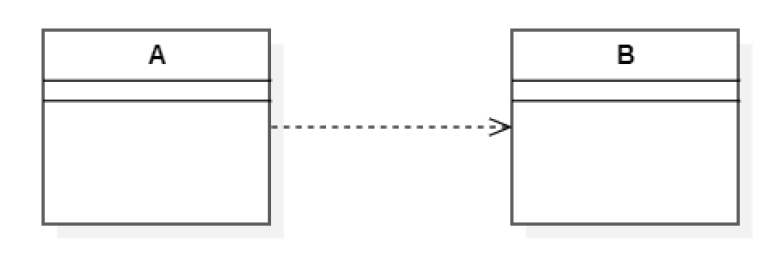
\includegraphics[width=0.5\linewidth]{img/dipendenza.PNG}
        \caption{Diagramma UML della relazione Dipendenza}
    \end{figure}
    
    \newpage
    
    \item \textbf{Composizione}
    \\La relazione di composizione tra due classi, A e B, implica che l'oggetto della classe A è composto da oggetti della classe B, e che l'esistenza degli oggetti della classe B dipende direttamente dall'esistenza degli oggetti della classe A. Questa relazione è rappresentata da una freccia solida con un rombo pieno alla fine, che punta dalla classe A alla classe B. 
    \begin{figure}[h]
        \centering
        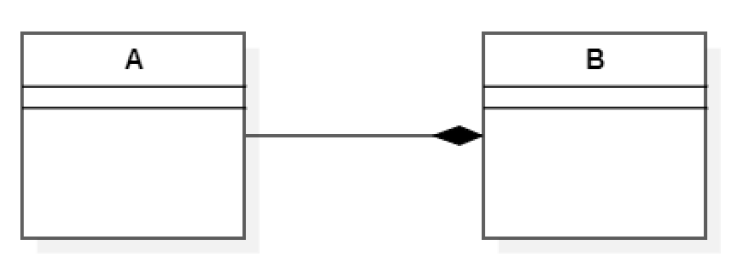
\includegraphics[width=0.5\linewidth]{img/composizione.PNG}
        \caption{Diagramma UML della relazione Composizione}
    \end{figure}
    
    
    
    \item \textbf{Aggregazione}
    \\La relazione di aggregazione tra due classi, A e B, implica che l'oggetto della classe A "aggrega" gli oggetti della classe B, ma questi ultimi possono esistere anche al di fuori del contesto della classe A. È rappresentata da una freccia con un rombo vuoto alla fine, che punta dalla classe A alla classe B. 
    \begin{figure}[h]
        \centering
        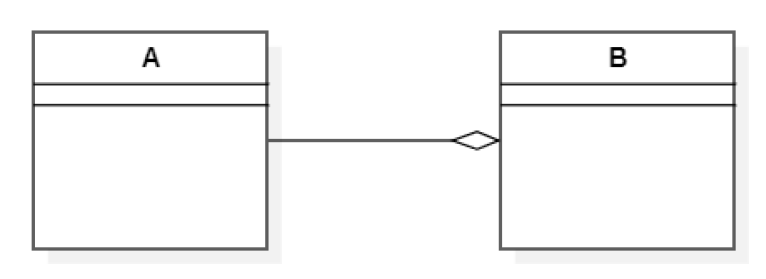
\includegraphics[width=0.5\linewidth]{img/aggregazione.PNG}
        \caption{Diagramma UML della relazione Aggregazione}
    \end{figure}

    
    \item \textbf{Relazione con interfaccia}
    \\La relazione con interfaccia tra due classi, A e B, è indicata da una linea non direzionata che collega la classe A a un cerchio vuoto che rappresenta l'interfaccia fornita dalla classe B. Questa relazione denota che la classe A dipende dall'interfaccia definita dalla classe B per specificare le sue operazioni, senza specificare l'implementazione concreta di tali operazioni. 
    \begin{figure}[h]
        \centering
        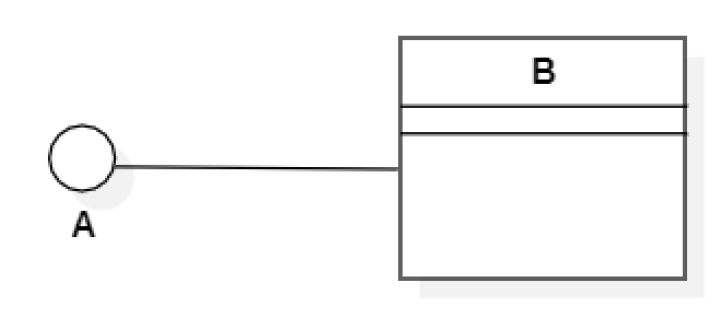
\includegraphics[width=0.5\linewidth]{img/interfaccia.PNG}
        \caption{Diagramma UML della relazione Interfaccia}
    \end{figure}
    
    
\end{itemize}

\subsubsubsection{Design Pattern}
I \textit{design patterns} sono soluzioni consolidate a problemi di progettazione che si presentano in modo ricorrente in diversi contesti. 
\\Questi modelli offrono un approccio riusabile alla progettazione, garantendo qualità nella soluzione e velocità nell'implementazione. 
\\L'adozione di un \textit{design pattern} avviene quando una soluzione si è dimostrata efficace in un contesto specifico, fornendo una guida affidabile per affrontare problemi simili in futuro. 
\\Di solito, vengono fornite dettagliate linee guida sull'applicazione dei pattern, insieme a una rappresentazione grafica e una spiegazione testuale della loro logica e utilità all'interno dell'$\textit{architettura}_G$ complessiva. 
\\Questa documentazione gioca un ruolo essenziale nel favorire la comprensione dell'integrazione del $\textit{design}_G$ pattern nell'$\textit{architettura}_G$ generale e nella prevenzione di errori di progettazione, assicurando coerenza e coesione nel $\textit{sistema}_G$ $\textit{software}_G$.

\subsubsubsection{Metriche}
\begin{longtable}{|>{\centering\arraybackslash}p{4cm}|p{7cm}|}
  \hline
  \rowcolor{gray!30}
  \textbf{Metrica} & \textbf{Nome} \\
  \hline
  \endfirsthead
  
  \rowcolor{gray!10}
    \begin{tabular}[c]{@{}c@{}}
        \textbf{MPD09-BS} \\
    \end{tabular}
  & \texttt{Browser supportati} \\
  \hline
  \rowcolor{gray!10}
    \begin{tabular}[c]{@{}c@{}}
        \textbf{MPD04-TA}
    \end{tabular}
     & \texttt{Tempo di apprendimento} \\
  \hline
  \rowcolor{gray!10}
    \begin{tabular}[c]{@{}c@{}}
        \textbf{MPD05-RO}
    \end{tabular}
     & \texttt{Raggiunta dell’obbiettivo} \\
  \hline
  \rowcolor{gray!10}
    \begin{tabular}[c]{@{}c@{}}
        \textbf{MPD06-EU}
    \end{tabular}
     & \texttt{Errori dell’utente} \\
  \hline
  \rowcolor{gray!10}
    \begin{tabular}[c]{@{}c@{}}
        \textbf{MPD03-TM}
    \end{tabular}
     & \texttt{Tempo di risposta medio} \\
  \hline
  \end{longtable}

\subsubsubsection{Strumenti}
\begin{itemize}
    \item \emph{\textbf{LucidChart}}: applicazione $\textit{software}_G$ utilizzata dal team per la realizzazione dei diagrammi riguardanti l'$\textit{architettura}_G$ logica.
    \item \emph{\textbf{StarUML}}: applicazione $\textit{software}_G$ utilizzata dal team per la realizzazione dei diagrammi delle classi.
\end{itemize}








\subsubsection{Codifica}
I programmatori, dopo l'analisi e la progettazione, implementano le funzionalità che deve avere il prodotto finale basandosi sull'\textit{Analisi Dei Requisiti} e sui documenti di progettazione.\\
Le aspettative riguardanti tale attività nel caso della $\textit{codifica}_G$ dell'$\textit{MVP}_G$ sono le seguenti:
\begin{itemize}
    \item  Le modifiche attuate dal programmatore devono essere coerenti con i requisiti e i casi d'uso presenti nel documento \textit{Analisi dei Requisiti}.
    Nel caso in cui fosse necessario rivedere alcuni sezioni si discute con l'analista su come procedere.
    \item Le modifiche attuate dal programmatore devono essere coerenti con l'$\textit{architettura}_G$ e la progettazione del documento \textit{Specifica Tecnica}. Nel caso in cui fosse necessario rivedere alcuni sezioni si discute con il progettista su come procedere.
    \item Rispetto a quanto implementato si devono inserire $\textit{test}_G$ di unità che assicurano il corretto funzionamento del prodotto.
\end{itemize}

\subsubsubsection{Norme di codifica}
Per la stesura del codice si sono adottate delle norme comuni tra cui:
\begin{itemize}
    \item \textbf{Convenzioni di denominazione}: Usare nomi significativi per variabili, funzioni, classi, ecc. usando opportunamente lettere maiuscole e minuscole per
    identificare le parole chiave.
    
    \item \textbf{Indentazione}: Usa l'indentazione in modo consistente per evidenziare la struttura del codice. 
    
    \item \textbf{Commenti}: Aggiungere commenti significativi per spiegare parti complesse del codice, ma evitare commenti ovvi o ridondanti. 
    
    \item \textbf{Lunghezza delle righe}: Limitare la lunghezza delle righe per una facile lettura e revisione del codice. 
    
    \item \textbf{Struttura del codice}: Organizzare il codice in blocchi logici e funzioni coese. Utilizzare funzioni e classi per evitare la duplicazione del codice.
    
    \item \textbf{Gestione delle eccezioni}: Trattare le eccezioni in modo appropriato, usando blocchi try\-catch quando necessario. Non ignorare mai le eccezioni senza gestirle.

     \item \textbf{Separare $\textit{logica di business}_G$ e logica di interfaccia}: Mantenere separata la $\textit{logica di business}_G$ dal codice di interfaccia utente o di accesso ai dati. Questo rende il codice più modulare e facile da testare.
\end{itemize}

\subsubsubsection{Metriche}
\begin{longtable}{|>{\centering\arraybackslash}p{4cm}|p{7cm}|}
  \hline
  \rowcolor{gray!30}
  \textbf{Metrica} & \textbf{Nome} \\
  \hline
  \endfirsthead
  
  \rowcolor{gray!10}
    \begin{tabular}[c]{@{}c@{}}
        \textbf{MPD08-CC} \\
    \end{tabular}
  & \texttt{Complessità ciclomatica} \\
  \hline
  \rowcolor{gray!10}
    \begin{tabular}[c]{@{}c@{}}
        \textbf{MPD07-FD}
    \end{tabular}
     & \texttt{Failure density} \\
  \hline
  \rowcolor{gray!10}
    \begin{tabular}[c]{@{}c@{}}
        \textbf{MPC15-PCTS}
    \end{tabular}
     & \texttt{Percentuale dei $\textit{test}_G$ superati} \\
  \hline
  \rowcolor{gray!10}
    \begin{tabular}[c]{@{}c@{}}
        \textbf{MPC16-SC}
    \end{tabular}
     & \texttt{Statement coverage} \\
  \hline
  \rowcolor{gray!10}
    \begin{tabular}[c]{@{}c@{}}
        \textbf{MPC17-BC}
    \end{tabular}
     & \texttt{Branch coverage} \\
  \hline
  \rowcolor{gray!10}
    \begin{tabular}[c]{@{}c@{}}
        \textbf{MPC18-CC}
    \end{tabular}
     & \texttt{Condition coverage} \\
  \hline
  \rowcolor{gray!10}
    \begin{tabular}[c]{@{}c@{}}
        \textbf{MPC12-LOC}
    \end{tabular}
     & \texttt{Linee di codice} \\
  \hline
  \end{longtable}



\subsubsubsection{Strumenti}
\begin{itemize}
    \item \emph{\textbf{Visual Studio Code}}: IDE utilizzato dal gruppo per la $\textit{codifica}_G$ del prodotto $\textit{software}_G$.
\end{itemize}